\makeatletter
\def\@copyrightspace{\relax}
\makeatother
\documentclass{report}
%\documentclass{article}

\begin{document}

\title{Odd Even Analysis}


\numberofauthors{2} 
\author{
\alignauthor
Niteesh Kumar Akurati\\
       \affaddr{IUB}\\
       \affaddr{F16-IG-3001}\\
       \affaddr{Bloomington,Indiana}\\
       \email{akuratin@umail.iu.edu}
\alignauthor
Parag Juneja\\
       \affaddr{IUB}\\
       \affaddr{F16-IG-3009}\\
       \affaddr{Bloomington,Indiana}\\
       \email{pjuneja@iu.edu}
}

\date{02 December 2016}


\maketitle
\begin{abstract}
Air pollution is an increasing concern across the globe. In densely populated mega cities of countries like India and China where the increasing vehicular density has become the major source of ambient air pollution. Most of these cities have not met air quality guidelines and have registered many number of deaths due to degraded air quality. Therefore, the Government of New Delhi has implemented a road rationing scheme called "Odd-Even Rule" to keep in check the rising pollution in Delhi. The scheme is a pilot project which is active for only 15 days (1st Jan,2016 to 15th Jan,2016) during which private cars are restricted movement based on their registration numbers. We analyzed the impact of this scheme in reducing the air pollution in Delhi.
\end{abstract}


\section{Introduction}
Air pollution is one of the major causes for the deaths in the world. The pollution caused by fine particles like particulate matter are directly affecting the health of the individuals. According to estimates 3 million deaths are caused due to outdoor air pollution annually around the globe. The particulate matter is a mixture of solid and liquid particles like smoke, dust, soot and liquid particles among which many are hazardous. The particulate matter is classified as PM2.5 and PM10 based on the size. The primary sources of this particulate matter are smoke from vehicles and industries. The air pollution is prominent in the densely-populated countries of the world like India and China where considering fast growing population and heavy increase of private vehicles for commute resulted in record high PM values especially in the major cities like New Delhi and Beijing. New Delhi is ranked as most polluted city in the world recently by WHO.

New Delhi is the capital city of India and the main center for major economic, political activities and an education hub which makes transportation more prominent within the city. The number of private vehicles used in the city is very high which leads to more air pollution. Vehicles being one of the major sources of particulate matter. To address this problem the government of New Delhi has piloted a pollution controlling project called the "Odd-Even Programmed" from January 1st, 2016 to January 15th, 2016. The program has put a restriction of movement on private cars by restricting the cars with odd numbered registration plates to odd numbered days and even numbered registration plates to even numbered days




\section{Problem Statement}
Air pollution is caused by several pollutants like PM2.5, PM10, Oxides of Nitrogen, Carbon Monoxide, Carbon Dioxide and several meteorological factors like wind, humidity, temperature etc. We as part of our analysis are considering the impact of the "Odd-Even Program" implemented in New Delhi. The program is concentrated across the vehicles. The prominent pollutants emitted by private cars that impact the environment are the particulate matter and nitrogen oxide. To perform a keen analysis of the impact of the program on the pollution levels in the New Delhi we observed the continuous monitoring data of the pollutants NO2 and PM2.5 available from the CPCB (Central Pollution Control Board), India monitoring stations. 

The reports in regards to the effect of the program on the pollution in the New Delhi were mixed as the result of program is abstract and cannot be exactly attributed to one factor. The success of the program can only be determined by observing the pollution levels within New Delhi and the areas which are closely located to New Delhi called the NCR (National Capital Region) and have the same pollution levels. The pollution is observed in both New Delhi and NCR region in two phases. In the first phase air pollution levels of both New Delhi and NCR are compared for the month December which is the pre-implementation phase of the odd-even program and in second phase we compared the air pollution levels of both New Delhi and NCR during the month January which is the month of the implementation of the odd-even program. This kind of approach is called the difference-in-difference analysis.
Through this analysis, we are hoping to provide some valuable insights in regards to the impact of this program on the air pollution of New Delhi during the implementation phase.\cite{CompleteStudyofFactorsContributingtoAirPollution} 

\section{Goals}
The main objectives of this analysis are: -

1) Studying the impact of pollutants NO2 and PM2.5 on the pollution and observing the dependencies

2)Compute the averages of pollutants (NO2 and PM2.5) of all the four stations in New Delhi on an hourly basis for both pre-implementation and during the implementation phase and compute the average of these four stations together for getting the mean average concentration for New Delhi

3)Compute the averages of Pollutants (NO2 and PM2.5) for Faridabad during the pre-implementation and post-implementation phases.

4)Apply the difference-in-difference analysis between New Delhi and Faridabad during each phase and observe the air pollution



\section{scope}
The scope of this analysis is:-

1)This analysis included data from five stations taken from CPCB(Central Pollution Control Board) out of them four of the stations are in New Delhi namely Anand Vihar, Punjabi Bagh, Mandir Marg, R K Puram and one is in the NCR region namely Faridabad.

2)The data collected for the analysis is for the duration of six months both hourly and monthly.

3)The primary goal of the analysis is to observe the air pollution in New Delhi during the implementation of "Odd-Even Program" using difference-in-differences methodology and provide substantial.

4)Given the short spectrum of the program which is 15 days we have limited size data-sets.


\section{Data Sources and Management}
The data used in the analysis is obtained from CPCB (Central Pollution Control Board) website. CPCB is a Government organization which keep tracks of about 20 pollutants using various monitoring stations installed by CPCB in various cities on  hourly and daily basis. But not all pollutants information is available at every station for every given hour. The major pollutants like NO2, PM2.5, SO2 and PM10 are now being tracked on a regular basis by CPCB. 

Based on the availability of the data we have taken four mostly polluted areas in New Delhi namely :-

1)Anandvihar

2)Mandir Marg

3)Punjabi Bagh 

4)R K Puram 

and data of one area in the NCR region namely :-

1)Faridabad.

The above mentioned stations in Delhi are taken because these regions either have dense population, more number of vehicles commuting on a average day and either located  in the interstate area.The data taken for these five stations are the pollutants NO2 and PM2.5 which are primarily emitted by the vehicles. The hourly data is collected for a total of 60 days which includes January and December months, these are the two phases of the analysis one is the pre-implementation phase and other is the during the implementation phase. Data is also collected for all the five stations for a period of 6 months to show how exactly the pollution is affected during different months of the year. 
 

\section{Data Preparation}
The data taken from the CPCB has information not recorded (or) missing for a number of days for certain pollutants. The missing data of different days is not taken into consideration.  The data is not treated for any missing values. The data for different months for different pollutants and different stations are available differently on the website.

The following steps describe the data preparation:-
1)The data for pollutant PM2.5 is taken for each individual station in Delhi and Faridabad.

2)There are many columns which are not required for the analysis those columns are dropped. 

3)The data from the five stations are taken and then combined manually into one comma separated values file called  hourly data of the pollutant PM2.5 


4)Similarly, the data for the pollutant NO2 is taken for each individual station in Delhi and Faridabad. 

5)The same procedure is applied for getting final csv file hourly data of the pollutant NO2 

\section{Tools}
For the purpose of doing Big Data analysis we have used the following tools:-

1)Python is used as a programming language for analysis

2)Excel is used for data preparation and analysis

3)Pandas library in python is used to get desired results from data

4)Numpy library in python is used for performing average calculations on the data

5)Online plotting tool plotly library for python to show various visualizations


\section{Problem Analysis Implemented}
The impact of the odd-even program implemented by government in New Delhi during January 1-15, 2016 is measured by performing multiple analysis which are discussed following in this section. 

An increase in pollution levels is observed both in Delhi and the surrounding area around Delhi, which is also known as NCR in January 2016 as compared to December 2015. But Delhi observed a smaller increase. We attribute this consequence to the Odd-Even program.

Main contributor to pollution, Particulate Matter(PM) has various sources. Weather conditions also affect the PM concentrations. It has been observed that low wind speeds and low temperatures lead to higher concentrations of PM. Therefore, increase in concentrations in January can be attributed to the weather conditions. Still we expect the pollutions levels to be lesser in comparison to what they would have been if the program was not implemented.

Data of the two major pollutants PM2.5 and NO2 whose contributions in pollution are colossal have been considered for analysis.

Program's impact on the pollution levels of Delhi has been inspected through following different analysis:

For the first analysis, monthly averages of concentrations of pollutants PM 2.5 and NO2 from the Delhi monitors (namely Anand Vihar, Mandir Marg, Punjabi Bagh, R K Puram), which are combined into one and the Faridabad monitor (part of NCR) are taken into consideration.


\graphicspath{ {report/} }
\includegraphics[width=8cm, height=7cm]{monthly_PM25}

For pollutant PM 2.5, as it can be clearly seen in line chart, if we look at monthly averages in the Delhi monitors and the Faridabad monitor from June 2015, we find that concentration levels increase equally for both Delhi and Faridabad. But in Jan 2016, concentration levels of PM2.5 increase considerably for Faridabad as compared to those for Delhi. Pollution levels within Delhi and areas close by outside Delhi like Faridabad should change in a similar way due to external factors like weather. Hence, any anomaly that is seen can be attributed to unalike factors like the odd-even program being implemented only in Delhi. 

\graphicspath{ {report/} }
\includegraphics[width=8cm, height=7cm]{monthly_NO2}

Similar analysis can be made in the case of pollutant NO2, whose concentration level decreases in Jan 2016 for Delhi as compared to Faridabad. 

For the second analysis, we look at hourly averages of concentrations of pollutants PM 2.5 and NO2 for the months of December 2015 and January 2016.

\graphicspath{ {report/} }
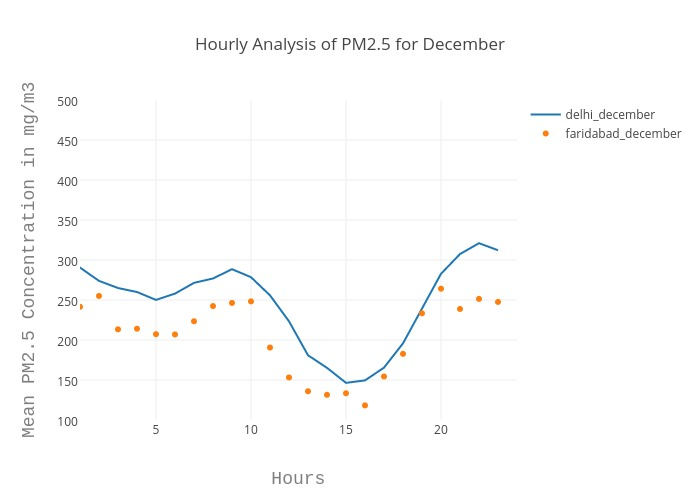
\includegraphics[width=8cm, height=7cm]{Linechart_December_PM25}

For pollutant PM 2.5, concentration levels in January are higher for both places Delhi and Faridabad. But levels of Faridabad clearly show more increase than those of Delhi.

\graphicspath{ {report/} }
\includegraphics[width=8cm, height=7cm]{Linechart_January_PM25}

Similar results can be observed for pollutant NO2.

\graphicspath{ {report/} }
\includegraphics[width=8cm, height=7cm]{Linechart_December_NO2}

Concentration levels of NO2 of Faridabad clearly show more increase than those of Delhi.

\graphicspath{ {report/} }
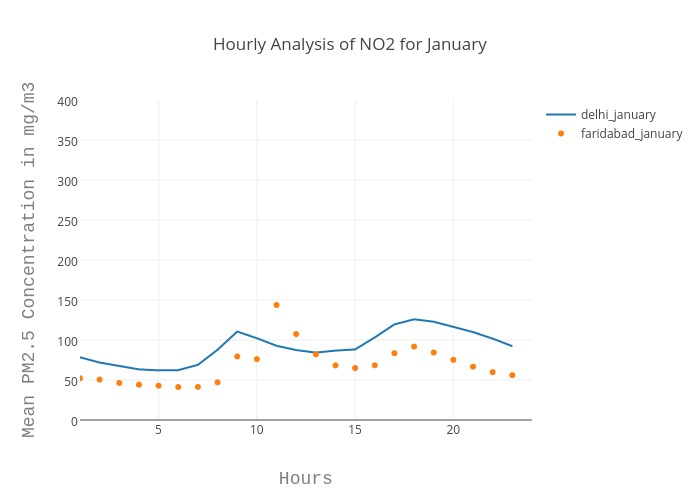
\includegraphics[width=8cm, height=7cm]{Linechart_January_NO2}

For the third analysis, a standard statistical technique called difference-in-differences is used:

Pollution data before and after the program both in the area where the program has been implemented and an appropriate adjoining area where the program has not been implemented is observed and compared.

%\begin{center}
\begin{tabular}{ | m{5em} | m{1cm}| m{1cm} | m{2.5cm} | } 
\hline
 & Before the program & After the program & Change during the time where program is implemented\\ 
\hline
Region where program is implemented & BP1 & AP1 & (AP1 - BP1) \\ 
\hline
Region where program is not implemented & BP2 & AP2 & (AP2 - BP2) \\ 
\hline
\end{tabular}
%\end{center}

\begin{tabular}{ |m{4cm} | m{2.9cm} | } 
\hline
Change due to program in the region where program is implemented & (AP1 - BP1) - (AP2 - BP2) \\ 
\hline
\end{tabular}

Because there can be some local factors that could change the pollution levels, for example in Delhi only its observed that Anand Vihar has a much bad air quality as compared to other place say Dwarka, therefore difference-in-differences proves to be an useful method to analyse the program impact on pollution levels. This is because it depends solely on the difference in changes as opposed to difference in absolute levels.\cite{Odd-Even-Program}

\graphicspath{ {report/} }
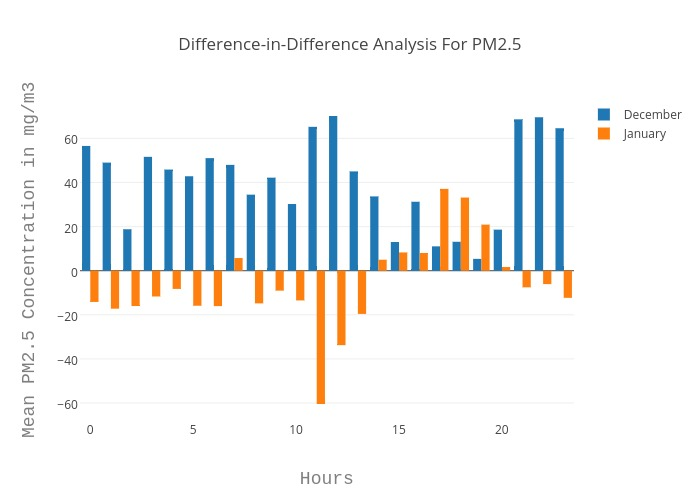
\includegraphics[width=8cm, height=7cm]{hourly_PM25}

We did the Difference in Differences analysis for pollutants PM2.5 and NO2 for the months of December and January. For the same we have subtracted the mean hourly concentrations of Faridabad from Delhi (considering  most polluted stations Anand Vihar, Mandir Marg, Punjabi Bagh and R K Puram). 

\graphicspath{ {report/} }
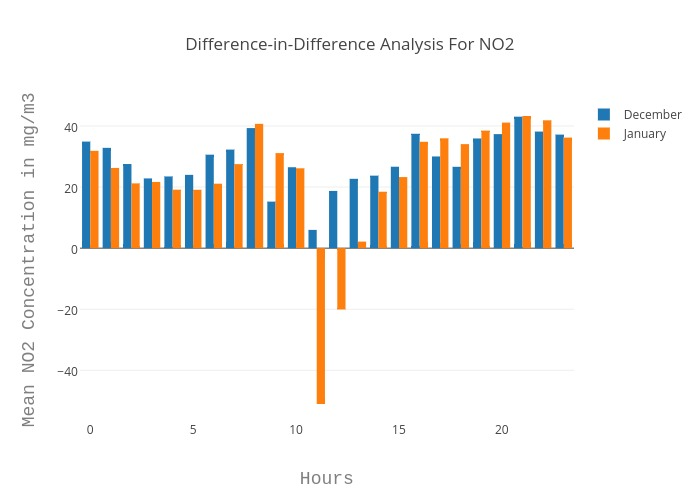
\includegraphics[width=8cm, height=7cm]{hourly_NO2}

As shown in the graphs, from the analysis, it can be clearly observed that Delhi minus Faridabad mean concentrations results of pollutants PM2.5 and NO2 for January are much lower than the month of December, which evidently proves our point that there was a considerable dip in the concentration levels of pollutants considered in the month of January 2016 for Delhi, which can be attributed to the odd even program implemented there. 

The odd-even program reduces pollution in two primary ways:-

i) There are fewer cars on the road which directly reduces the levels of pollutants like PM2.5 and NO2.

ii) Reduced congestion also reduces idling and slow moving traffic across the city, thereby also reducing pollution in the capital.

\section{Work Breakdown}

Tasks done by Parag Juneja :-

a) Project Idea and Proposal.

   Came up with the idea of the project and proposed what could be the scope of the project.
   
b) Fetching Data
 
   Downloaded hourly data of pollutant NO2 for the months December 2015 and January 2016 from Central Pollution Control Board website.
   
   Also, downloaded the monthly data of pollutants PM2.5 and NO2 for the months June15, July15, August15, September15, October15, November15, December15 and January16 from Central Pollution Control Board website.
 
c) Data Cleanup

   Extracted all the useful data from the data-sets downloaded and arranged them into useful form.
  
d) Code

   Implemented the code for difference in differences analysis for pollutants PM2.5 and NO2.
   
   Also, implemented the code for monthly analysis of concentrations of pollutants PM2.5 and NO2.
   
e) Report

   Contributed in authoring the report for the project.
   

Tasks done by Niteesh Kumar Akurati :- 

a) Domain analysis and Scope.

   Did the domain analysis, confirmed the feasibility and defined the scope of the project.
   
b) Fetching Data
 
   Downloaded hourly data of pollutant PM2.5 for the months December 2015 and January 2016 from Central Pollution Control Board website.
    
c) Data Cleanup

   Extracted all the useful data from the data-sets downloaded and arranged them into useful form.
  
d) Code

   Implemented the code for hourly analysis of concentrations of pollutants PM2.5 and NO2 for the months of December 2015 and January 2016.
   
e) Report

   Contributed in authoring the report for the project

\section{Conclusion}

With the help of the results generated by the three analysis performed as mentioned in Problem Analysis Implemented section we conclude that Odd-Even program implemented by the Delhi government from January 1 2016 - January 15 2016 was indeed successful in achieving its desired goal of reducing the pollution in the capital of India, New Delhi. 

\bibliographystyle{abbrv}
\bibliography{references}

%\balancecolumns 

\end{document}
